%\renewcommand{\theequation}{\theenumi}
%\begin{enumerate}[label=\arabic*.,ref=\theenumi]
\begin{enumerate}[label=\thesection.\arabic*.,ref=\thesection.\theenumi]
\numberwithin{equation}{enumi}
\item Suppose the equations $AB, BC$ and $CA$ are respectively given by 
		\begin{align}
			\label{eq:tri-sides}
			\vec{n}_i^{\top}\vec{x}=c_i \quad i = 1, 2, 3 
		\end{align}
		The equations of the respective angle bisectors are then given by 
		\begin{align}
			\frac{\vec{n}_i^{\top}\vec{x}-c_i}{\norm{\vec{n}_i}}
		=
	\pm	\frac{\vec{n}_j^{\top}\vec{x}-c_j}{\norm{\vec{n}_j}}
\quad i \ne j
		\end{align}
		Substitute numerical values and find the equations of the angle bisectors of $A, B$ and $C$.
	\\
		%\iffalse
\let\negmedspace\undefined
\let\negthickspace\undefined
\documentclass[journal,12pt,twocolumn]{IEEEtran}
\usepackage{cite}
\usepackage{amsmath,amssymb,amsfonts,amsthm}
\usepackage{algorithmic}
\usepackage{graphicx}
\usepackage{textcomp}
\usepackage{xcolor}
\usepackage{txfonts}
\usepackage{listings}
\usepackage{enumitem}
\usepackage{mathtools}
\usepackage{gensymb}
\usepackage[breaklinks=true]{hyperref}
\usepackage{tkz-euclide} % loads  TikZ and tkz-base
\usepackage{listings}
\usepackage{gvv}
%
%\usepackage{setspace}
%\usepackage{gensymb}
%\doublespacing
%\singlespacing

%\usepackage{graphicx}
%\usepackage{amssymb}
%\usepackage{relsize}
%\usepackage[cmex10]{amsmath}
%\usepackage{amsthm}
%\interdisplaylinepenalty=2500
%\savesymbol{iint}
%\usepackage{txfonts}
%\restoresymbol{TXF}{iint}
%\usepackage{wasysym}
%\usepackage{amsthm}
%\usepackage{iithtlc}
%\usepackage{mathrsfs}
%\usepackage{txfonts}
%\usepackage{stfloats}
%\usepackage{bm}
%\usepackage{cite}
%\usepackage{cases}
%\usepackage{subfig}
%\usepackage{xtab}
%\usepackage{longtable}
%\usepackage{multirow}
%\usepackage{algorithm}
%\usepackage{algpseudocode}
%\usepackage{enumitem}
%\usepackage{mathtools}
%\usepackage{tikz}
%\usepackage{circuitikz}
%\usepackage{verbatim}
%\usepackage{tfrupee}
%\usepackage{stmaryrd}
%\usetkzobj{all}
%    \usepackage{color}                                            %%
%    \usepackage{array}                                            %%
%    \usepackage{longtable}                                        %%
%    \usepackage{calc}                                             %%
%    \usepackage{multirow}                                         %%
%    \usepackage{hhline}                                           %%
%    \usepackage{ifthen}                                           %%
  %optionally (for landscape tables embedded in another document): %%
%    \usepackage{lscape}     
%\usepackage{multicol}
%\usepackage{chngcntr}
%\usepackage{enumerate}

%\usepackage{wasysym}
%\documentclass[conference]{IEEEtran}
%\IEEEoverridecommandlockouts
% The preceding line is only needed to identify funding in the first footnote. If that is unneeded, please comment it out.

\newtheorem{theorem}{Theorem}[section]
\newtheorem{problem}{Problem}
\newtheorem{proposition}{Proposition}[section]
\newtheorem{lemma}{Lemma}[section]
\newtheorem{corollary}[theorem]{Corollary}
\newtheorem{example}{Example}[section]
\newtheorem{definition}[problem]{Definition}
%\newtheorem{thm}{Theorem}[section] 
%\newtheorem{defn}[thm]{Definition}
%\newtheorem{algorithm}{Algorithm}[section]
%\newtheorem{cor}{Corollary}
\newcommand{\BEQA}{\begin{eqnarray}}
\newcommand{\EEQA}{\end{eqnarray}}
\newcommand{\define}{\stackrel{\triangle}{=}}
\theoremstyle{remark}
\newtheorem{rem}{Remark}

%\bibliographystyle{ieeetr}
\begin{document}
%

\bibliographystyle{IEEEtran}


\vspace{3cm}

\title{
%	\logo{
ASSIGNMENT-1
%	}
}
\author{ RAMBHA SATVIK - EE22BTECH11043$^{*}$% <-this % stops a space
	\thanks{*The author is with the Department
		of Electrical Engineering, Indian Institute of Technology, Hyderabad
		502285 India e-mail:  ee22btech11043@iith.ac.in. All content in this manual is released under GNU GPL.  Free and open source.}
	
}	
%\title{
%	\logo{Matrix Analysis through Octave}{\begin{center}\includegraphics[scale=.24]{tlc}\end{center}}{}{HAMDSP}
%}


% paper title
% can use linebreaks \\ within to get better formatting as desired
%\title{Matrix Analysis through Octave}
%
%
% author names and IEEE memberships
% note positions of commas and nonbreaking spaces ( ~ ) LaTeX will not break
% a structure at a ~ so this keeps an author's name from being broken across
% two lines.
% use \thanks{} to gain access to the first footnote area
% a separate \thanks must be used for each paragraph as LaTeX2e's \thanks
% was not built to handle multiple paragraphs
%

%\author{<-this % stops a space
%\thanks{}}
%}
% note the % following the last \IEEEmembership and also \thanks - 
% these prevent an unwanted space from occurring between the last author name
% and the end of the author line. i.e., if you had this:
% 
% \author{....lastname \thanks{...} \thanks{...} }
%                     ^------------^------------^----Do not want these spaces!
%
% a space would be appended to the last name and could cause every name on that
% line to be shifted left slightly. This is one of those "LaTeX things". For
% instance, "\textbf{A} \textbf{B}" will typeset as "A B" not "AB". To get
% "AB" then you have to do: "\textbf{A}\textbf{B}"
% \thanks is no different in this regard, so shield the last } of each \thanks
% that ends a line with a % and do not let a space in before the next \thanks.
% Spaces after \IEEEmembership other than the last one are OK (and needed) as
% you are supposed to have spaces between the names. For what it is worth,
% this is a minor point as most people would not even notice if the said evil
% space somehow managed to creep in.



% The paper headers
%\markboth{Journal of \LaTeX\ Class Files,~Vol.~6, No.~1, January~2007}%
%{Shell \MakeLowercase{\textit{et al.}}: Bare Demo of IEEEtran.cls for Journals}
% The only time the second header will appear is for the odd numbered pages
% after the title page when using the twoside option.
% 
% *** Note that you probably will NOT want to include the author's ***
% *** name in the headers of peer review papers.                   ***
% You can use \ifCLASSOPTIONpeerreview for conditional compilation here if
% you desire.




% If you want to put a publisher's ID mark on the page you can do it like
% this:
%\IEEEpubid{0000--0000/00\$00.00~\copyright~2007 IEEE}
% Remember, if you use this you must call \IEEEpubidadjcol in the second
% column for its text to clear the IEEEpubid mark.



% make the title area
\maketitle

\newpage

%\tableofcontents

\bigskip

\renewcommand{\thefigure}{\theenumi}
\renewcommand{\thetable}{\theenumi}
%\renewcommand{\theequation}{\theenumi}

%\begin{abstract}
%%\boldmath
%In this letter, an algorithm for evaluating the exact analytical bit error rate  (BER)  for the piecewise linear (PL) combiner for  multiple relays is presented. Previous results were available only for upto three relays. The algorithm is unique in the sense that  the actual mathematical expressions, that are prohibitively large, need not be explicitly obtained. The diversity gain due to multiple relays is shown through plots of the analytical BER, well supported by simulations. 
%
%\end{abstract}
% IEEEtran.cls defaults to using nonbold math in the Abstract.
% This preserves the distinction between vectors and scalars. However,
% if the journal you are submitting to favors bold math in the abstract,
% then you can use LaTeX's standard command \boldmath at the very start
% of the abstract to achieve this. Many IEEE journals frown on math
% in the abstract anyway.

% Note that keywords are not normally used for peerreview papers.
%\begin{IEEEkeywords}
%Cooperative diversity, decode and forward, piecewise linear
%\end{IEEEkeywords}



% For peer review papers, you can put extra information on the cover
% page as needed:
% \ifCLASSOPTIONpeerreview
% \begin{center} \bfseries EDICS Category: 3-BBND \end{center}
% \fi
%
% For peerreview papers, this IEEEtran command inserts a page break and
% creates the second title. It will be ignored for other modes.
%\IEEEpeerreviewmaketitle

\textbf{Question :} Suppose the equations \textit{AB, BC} and \textit{CA} are respectively given by
		\begin{align}
			\vec{n}_{i}^{\top} \vec{x} = c_{i} \hspace{0.25in} i = 1,2,3
		\end{align}
		The equations of the respective angle bisectors are given by
		\begin{align}
			\frac{\vec{n}_{i}^{\top} \vec{x}-c_{i}}{\norm{\vec{n}_{i}}}=\pm\frac{\vec{n}_{j}^{\top} \vec{x}-c_{j}}{\norm{\vec{n}_{j}}} \hspace{0.25in}i\neq j 
		\end{align}
		Substitute numerical values and find the equations of the angle bisectors of \textit{A,B} and \textit{C}.\\
\fi
\textbf{Solution :}
	The parametric equations of sides;
	\begin{align}
	BC:\quad &\myvec{11&1}\vec{x}=-38,\\
	CA:\quad &\myvec{1&-1}\vec{x}=2,\\
	AB:\quad &\myvec{7&5}\vec{x}=2\\	  
	\end{align}
	Using the formula mentioned in the question to find out the angular bisector for sides \text{AB} and \text{AC}, naming the angular bisector $L$ we get,
	\begin{align}
		\frac{\vec{n}_{3}^{\top} \vec{x}-c_{3}}{\norm{\vec{n}_{3}}}=\pm \frac{\vec{n}_{2}^{\top} \vec{x}-c_{2}}{\norm{\vec{n}_{2}}}
	\end{align}
	\begin{figure}
	\centering
	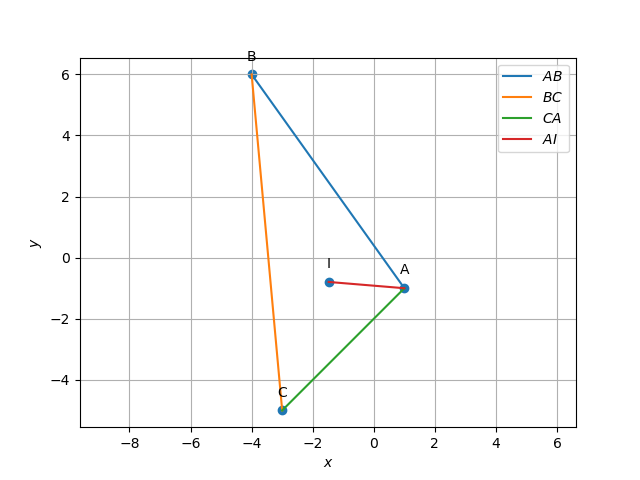
\includegraphics[width=\columnwidth]{solutions/1/5/1/figs/angular_bisector.png}
	\caption{Triangle generated using python}
	\label{fig:angular_bisector}
	\end{figure}
	As we can see we will get 2 solutions for $L$. This is because one of them is internal angular bisector and the other is the external angular bisector. Internal angular bisector can be evaluated if we take + in the above formula.
	Hence, $L$ is given by,
	\begin{align}
		\frac{\vec{n}_{3}^{\top} \vec{x}-c_{3}}{\norm{\vec{n}_{3}}}&=\frac{\vec{n}_{2}^{\top} \vec{x}-c_{2}}{\norm{\vec{n}_{2}}}\\
		\implies \brak{\frac{\vec{n_{3}}}{\norm{\vec{n_{3}}}}-\frac{\vec{n_{3}}}{\norm{\vec{n_{3}}}}} \vec{x}&=\brak{\frac{c_{3}}{\norm{\vec{n_{3}}}}-\frac{c_{2}}{\norm{\vec{n_{2}}}}}\\
		\implies \brak{\frac{\myvec{7&5}}{\sqrt{74}}-\frac{\myvec{1&-1}}{\sqrt{2}}} \vec{x}&=\frac{2}{\sqrt{74}}-\frac{2}{\sqrt{2}}\\
		\implies \myvec{\frac{7-\sqrt{37}}{\sqrt{74}}&\frac{5+\sqrt{37}}{\sqrt{74}}}\vec{x}&=\frac{2-2\sqrt{37}}{\sqrt{74}}
	\end{align}
	Hence, the internal angluar bisector of angle $A$, $L$ will be,
	\begin{align}
		\implies\myvec{\frac{7-\sqrt{37}}{\sqrt{74}}&\frac{5+\sqrt{37}}{\sqrt{74}}} \vec{x}=\frac{2-2\sqrt{37}}{\sqrt{74}}
		\label{eq:1.5.1}
	\end{align}
	

  \iffalse
\documentclass[journal,12pt,twocolumn]{IEEEtran}
\usepackage{cite}
\usepackage{amsmath,amssymb,amsfonts,amsthm}
\usepackage{algorithmic}
\usepackage{graphicx}
\usepackage{textcomp}
\usepackage{xcolor}
\usepackage{txfonts}
\usepackage{listings}
\usepackage{enumitem}
\usepackage{mathtools}
\usepackage{gensymb}
\usepackage[breaklinks=true]{hyperref}
\usepackage{tkz-euclide} % loads  TikZ and tkz-base
\usepackage{listings}
\usepackage{float}


\begin{document}
\providecommand{\pr}[1]{\ensuremath{\Pr\left(#1\right)}}
\providecommand{\prt}[2]{\ensuremath{p_{#1}^{\left(#2\right)} }}        % own macro for this question
\providecommand{\qfunc}[1]{\ensuremath{Q\left(#1\right)}}
\providecommand{\sbrak}[1]{\ensuremath{{}\left[#1\right]}}
\providecommand{\lsbrak}[1]{\ensuremath{{}\left[#1\right.}}
\providecommand{\rsbrak}[1]{\ensuremath{{}\left.#1\right]}}
\providecommand{\brak}[1]{\ensuremath{\left(#1\right)}}
\providecommand{\lbrak}[1]{\ensuremath{\left(#1\right.}}
\providecommand{\rbrak}[1]{\ensuremath{\left.#1\right)}}
\providecommand{\cbrak}[1]{\ensuremath{\left\{#1\right\}}}
\providecommand{\lcbrak}[1]{\ensuremath{\left\{#1\right.}}
\providecommand{\rcbrak}[1]{\ensuremath{\left.#1\right\}}}
\newcommand{\sgn}{\mathop{\mathrm{sgn}}}
\providecommand{\abs}[1]{\left\vert#1\right\vert}
\providecommand{\res}[1]{\Res\displaylimits_{#1}} 
\providecommand{\norm}[1]{\left\lVert#1\right\rVert}
%\providecommand{\norm}[1]{\lVert#1\rVert}
\providecommand{\mtx}[1]{\mathbf{#1}}
\providecommand{\mean}[1]{E\left[ #1 \right]}
\providecommand{\cond}[2]{#1\middle|#2}
\providecommand{\fourier}{\overset{\mathcal{F}}{ \rightleftharpoons}}
\newenvironment{amatrix}[1]{%
  \left(\begin{array}{@{}*{#1}{c}|c@{}}
}{%
  \end{array}\right)
}
%\providecommand{\hilbert}{\overset{\mathcal{H}}{ \rightleftharpoons}}
%\providecommand{\system}{\overset{\mathcal{H}}{ \longleftrightarrow}}
	%\newcommand{\solution}[2]{\textbf{Solution:}{#1}}
\newcommand{\solution}{\noindent \textbf{Solution: }}
\newcommand{\cosec}{\,\text{cosec}\,}
\providecommand{\dec}[2]{\ensuremath{\overset{#1}{\underset{#2}{\gtrless}}}}
\newcommand{\myvec}[1]{\ensuremath{\begin{pmatrix}#1\end{pmatrix}}}
\newcommand{\mydet}[1]{\ensuremath{\begin{vmatrix}#1\end{vmatrix}}}
\newcommand{\myaugvec}[2]{\ensuremath{\begin{amatrix}{#1}#2\end{amatrix}}}
\providecommand{\rank}{\text{rank}}
\providecommand{\pr}[1]{\ensuremath{\Pr\left(#1\right)}}
\providecommand{\qfunc}[1]{\ensuremath{Q\left(#1\right)}}
	\newcommand*{\permcomb}[4][0mu]{{{}^{#3}\mkern#1#2_{#4}}}
\newcommand*{\perm}[1][-3mu]{\permcomb[#1]{P}}
\newcommand*{\comb}[1][-1mu]{\permcomb[#1]{C}}
\providecommand{\qfunc}[1]{\ensuremath{Q\left(#1\right)}}
\providecommand{\gauss}[2]{\mathcal{N}\ensuremath{\left(#1,#2\right)}}
\providecommand{\diff}[2]{\ensuremath{\frac{d{#1}}{d{#2}}}}
\providecommand{\myceil}[1]{\left \lceil #1 \right \rceil }
\newcommand\figref{Fig.~\ref}
\newcommand\tabref{Table~\ref}
\newcommand{\sinc}{\,\text{sinc}\,}
\newcommand{\rect}{\,\text{rect}\,}
%%
%	%\newcommand{\solution}[2]{\textbf{Solution:}{#1}}
%\newcommand{\solution}{\noindent \textbf{Solution: }}
%\newcommand{\cosec}{\,\text{cosec}\,}
%\numberwithin{equation}{section}
%\numberwithin{equation}{subsection}
%\numberwithin{problem}{section}
%\numberwithin{definition}{section}
%\makeatletter
%\@addtoreset{figure}{problem}
%\makeatother

%\let\StandardTheFigure\thefigure
\let\vec\mathbf

\bibliographystyle{IEEEtran}


\vspace{3cm}

\textbf{Question 1.5.1}\\
Suppose the equations $AB, BC$ and $CA$ are respectively given by 
		\begin{align}
			\label{eq:tri-sides}
			\vec{n}_i^{\top}\vec{x}=c_i \quad i = 1, 2, 3 
		\end{align}
		The equations of the respective angle bisectors are then given by 
		\begin{align}
			\frac{\vec{n}_i^{\top}\vec{x}-c_i}{\norm{\vec{n}_i}}
		=
	\pm	\frac{\vec{n}_j^{\top}\vec{x}-c_j}{\norm{\vec{n}_j}}
\quad i \ne j
		\end{align}
		Substitute numerical values and find the equations of the angle bisectors of $A, B$ and $C$.\\
\fi
\solution 
The internal angle bisector is obtained from the set of two bisectors by using:
		\begin{align}
			\frac{\vec{n}_i^{\top}\vec{x}-c_i}{\norm{\vec{n}_i}}
		=
		\frac{\vec{n}_j^{\top}\vec{x}-c_j}{\norm{\vec{n}_j}}
\quad i \ne j	
\end{align}
This can be transformed to the normal equation of angle bisectors as follows 
\begin{align}
       \myvec{\frac{\vec{n}_i^{\top}}{\norm{\vec{n}_i}} - \frac{\vec{n}_j^{\top}}{\norm{\vec{n}_j}}}\vec{x}
       =
       \frac{c_i}{\norm{\vec{n}_i}}-\frac{c_j}{\norm{\vec{n}_j}}
\end{align}
$i$ and $j$ values correspond to the sides including the angle\\
\begin{enumerate}
\item Angle Bisector of $A$
\begin{align}
       \myvec{\frac{\vec{n}_3^{\top}}{\norm{\vec{n}_3}} - \frac{\vec{n}_1^{\top}}{\norm{\vec{n}_1}}}\vec{x}
       =
       \frac{c_3}{\norm{\vec{n}_3}}-\frac{c_1}{\norm{\vec{n}_1}}
\end{align}
on substitution we obtain 
\begin{align}
\myvec{
\frac{7}{\sqrt{74}}-\frac{1}{\sqrt{2}} & \frac{5}{\sqrt{74}}+\frac{1}{\sqrt{2}}\\
}
\vec{x}
=\frac{2}{\sqrt{74}}-\frac{2}{\sqrt{2}}
\end{align}
\item Angle Bisector of $B$
\begin{align}
       \myvec{\frac{\vec{n}_2^{\top}}{\norm{\vec{n}_2}} - \frac{\vec{n}_1^{\top}}{\norm{\vec{n}_1}}}\vec{x}
       =
       \frac{c_2}{\norm{\vec{n}_2}}-\frac{c_1}{\norm{\vec{n}_1}}
\end{align}
on substitution we obtain 
\begin{align}
\myvec{
\frac{11}{\sqrt{122}}+\frac{7}{\sqrt{74}} & \frac{1}{\sqrt{122}}+\frac{5}{\sqrt{74}}\\
}
\vec{x}
=\frac{2}{\sqrt{74}}-\frac{38}{\sqrt{122}}
\end{align}
\item Angle Bisector of $C$
\begin{align}
       \myvec{\frac{\vec{n}_2^{\top}}{\norm{\vec{n}_2}} - \frac{\vec{n}_3^{\top}}{\norm{\vec{n}_3}}}\vec{x}
       =
       \frac{c_2}{\norm{\vec{n}_2}}-\frac{c_3}{\norm{\vec{n}_3}}
\end{align}
on substitution we obtain 
\begin{align}
\myvec{
\frac{11}{\sqrt{122}}+\frac{1}{\sqrt{2}} & \frac{1}{\sqrt{122}}-\frac{1}{\sqrt{2}}\\
}
\vec{x}
=\frac{2}{\sqrt{2}}-\frac{38}{\sqrt{122}}
\end{align}
\end{enumerate}
\begin{figure}[H]
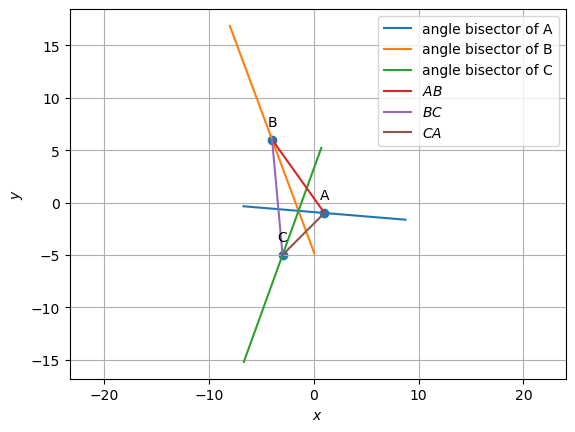
\includegraphics[width=\columnwidth]{./figs/anglebisector.png}
\caption{Angle bisectors plotted using python}
\label{fig:i_angbisector_py}
\end{figure}

	\item Find the intersection $\vec{I}$ of the angle bisectors of $B$ and $C$.
 \\
		\documentclass[journal,12pt,twocolumn]{IEEEtran}
\usepackage{cite}
\usepackage{amsmath,amssymb,amsfonts,amsthm}
\usepackage{algorithmic}
\usepackage{graphicx}
\usepackage{textcomp}
\usepackage{xcolor}
\usepackage{txfonts}
\usepackage{listings}
\usepackage{enumitem}
\usepackage{mathtools}
\usepackage{gensymb}
\usepackage[breaklinks=true]{hyperref}
\usepackage{tkz-euclide} % loads  TikZ and tkz-base
\usepackage{listings}
\usepackage{float}


\begin{document}
\providecommand{\pr}[1]{\ensuremath{\Pr\left(#1\right)}}
\providecommand{\prt}[2]{\ensuremath{p_{#1}^{\left(#2\right)} }}        % own macro for this question
\providecommand{\qfunc}[1]{\ensuremath{Q\left(#1\right)}}
\providecommand{\sbrak}[1]{\ensuremath{{}\left[#1\right]}}
\providecommand{\lsbrak}[1]{\ensuremath{{}\left[#1\right.}}
\providecommand{\rsbrak}[1]{\ensuremath{{}\left.#1\right]}}
\providecommand{\brak}[1]{\ensuremath{\left(#1\right)}}
\providecommand{\lbrak}[1]{\ensuremath{\left(#1\right.}}
\providecommand{\rbrak}[1]{\ensuremath{\left.#1\right)}}
\providecommand{\cbrak}[1]{\ensuremath{\left\{#1\right\}}}
\providecommand{\lcbrak}[1]{\ensuremath{\left\{#1\right.}}
\providecommand{\rcbrak}[1]{\ensuremath{\left.#1\right\}}}
\newcommand{\sgn}{\mathop{\mathrm{sgn}}}
\providecommand{\abs}[1]{\left\vert#1\right\vert}
\providecommand{\res}[1]{\Res\displaylimits_{#1}} 
\providecommand{\norm}[1]{\left\lVert#1\right\rVert}
%\providecommand{\norm}[1]{\lVert#1\rVert}
\providecommand{\mtx}[1]{\mathbf{#1}}
\providecommand{\mean}[1]{E\left[ #1 \right]}
\providecommand{\cond}[2]{#1\middle|#2}
\providecommand{\fourier}{\overset{\mathcal{F}}{ \rightleftharpoons}}
\newenvironment{amatrix}[1]{%
  \left(\begin{array}{@{}*{#1}{c}|c@{}}
}{%
  \end{array}\right)
}
%\providecommand{\hilbert}{\overset{\mathcal{H}}{ \rightleftharpoons}}
%\providecommand{\system}{\overset{\mathcal{H}}{ \longleftrightarrow}}
	%\newcommand{\solution}[2]{\textbf{Solution:}{#1}}
\newcommand{\solution}{\noindent \textbf{Solution: }}
\newcommand{\cosec}{\,\text{cosec}\,}
\providecommand{\dec}[2]{\ensuremath{\overset{#1}{\underset{#2}{\gtrless}}}}
\newcommand{\myvec}[1]{\ensuremath{\begin{pmatrix}#1\end{pmatrix}}}
\newcommand{\mydet}[1]{\ensuremath{\begin{vmatrix}#1\end{vmatrix}}}
\newcommand{\myaugvec}[2]{\ensuremath{\begin{amatrix}{#1}#2\end{amatrix}}}
\providecommand{\rank}{\text{rank}}
\providecommand{\pr}[1]{\ensuremath{\Pr\left(#1\right)}}
\providecommand{\qfunc}[1]{\ensuremath{Q\left(#1\right)}}
	\newcommand*{\permcomb}[4][0mu]{{{}^{#3}\mkern#1#2_{#4}}}
\newcommand*{\perm}[1][-3mu]{\permcomb[#1]{P}}
\newcommand*{\comb}[1][-1mu]{\permcomb[#1]{C}}
\providecommand{\qfunc}[1]{\ensuremath{Q\left(#1\right)}}
\providecommand{\gauss}[2]{\mathcal{N}\ensuremath{\left(#1,#2\right)}}
\providecommand{\diff}[2]{\ensuremath{\frac{d{#1}}{d{#2}}}}
\providecommand{\myceil}[1]{\left \lceil #1 \right \rceil }
\newcommand\figref{Fig.~\ref}
\newcommand\tabref{Table~\ref}
\newcommand{\sinc}{\,\text{sinc}\,}
\newcommand{\rect}{\,\text{rect}\,}
%%
%	%\newcommand{\solution}[2]{\textbf{Solution:}{#1}}
%\newcommand{\solution}{\noindent \textbf{Solution: }}
%\newcommand{\cosec}{\,\text{cosec}\,}
%\numberwithin{equation}{section}
%\numberwithin{equation}{subsection}
%\numberwithin{problem}{section}
%\numberwithin{definition}{section}
%\makeatletter
%\@addtoreset{figure}{problem}
%\makeatother

%\let\StandardTheFigure\thefigure
\let\vec\mathbf

\bibliographystyle{IEEEtran}


\vspace{3cm}

Question 1.5.2\\
Find the intersection $\vec{I}$ of the angle bisectors of $\vec{B}$ and $\vec{C}$
\fi
Solution:\\
From \ref{eq:1.5.1} the bisectors of $\vec{B}$ and $\vec{C}$ are obtained as 
\begin{align}
\myvec{
\frac{11}{\sqrt{122}}+\frac{7}{\sqrt{74}} & \frac{1}{\sqrt{122}}+\frac{5}{\sqrt{74}}\\
}
\vec{x}
=\frac{2}{\sqrt{74}}-\frac{38}{\sqrt{122}}
\end{align}
and 
\begin{align}
\myvec{
\frac{11}{\sqrt{122}}+\frac{1}{\sqrt{2}} & \frac{1}{\sqrt{122}}-\frac{1}{\sqrt{2}}\\
}
\vec{x}
=\frac{2}{\sqrt{2}}-\frac{38}{\sqrt{122}}
\end{align}
respectively.
The pair of linear equations can be solved using the Augmented matrix $\myvec{
\vec{P}|\vec{Q}}$
Here,
\begin{align}
\vec{P}&=\myvec{
\frac{11}{\sqrt{122}}+\frac{7}{\sqrt{74}} & \frac{1}{\sqrt{122}}+\frac{5}{\sqrt{74}}\\
\frac{11}{\sqrt{122}}+\frac{1}{\sqrt{2}} & \frac{1}{\sqrt{122}}-\frac{1}{\sqrt{2}}\\
}\\
\vec{Q}&=\myvec{
\frac{2}{\sqrt{74}}-\frac{38}{\sqrt{122}}\
\frac{2}{\sqrt{2}}-\frac{38}{\sqrt{122}}\\
}\\
\myaugvec{1}{\vec{P}&\vec{Q}} 
 &= \myaugvec{2}
 {
\frac{11}{\sqrt{122}}+\frac{7}{\sqrt{74}} & \frac{1}{\sqrt{122}}+\frac{5}{\sqrt{74}} & \frac{2}{\sqrt{74}}-\frac{38}{\sqrt{122}} \\
\frac{11}{\sqrt{122}}+\frac{1}{\sqrt{2}} & \frac{1}{\sqrt{122}}-\frac{1}{\sqrt{2}} & \frac{2}{\sqrt{2}}-\frac{38}{\sqrt{122}} \\
}
\end{align}
The augmented matrix is converted into decimal notations for easier calculations and then can be solved using row reduction as follows 
\begin{align}
\myaugvec{2}
{
1.81 & 0.67 & -3.21 \\
 1.7 & -0.62 & -2.03\\
}
 \xleftrightarrow[]{R_2\leftarrow 1.7R_1-1.81R_2}
\myaugvec{2}
{1.81 & 0.67 & -3.21 \\
0 & 1.33 & -1.05\\
}\\
\xleftrightarrow[]{R_1\leftarrow 1.33R_1-0.67R_2}
\myaugvec{2}
{1.81 & 0 & -2.68 \\
0 & 1.33 & -1.05\\
}\\
\xleftrightarrow[]{R_1\leftarrow \frac{R_1}{1.81}}
\myaugvec{2}
{
1 & 0 & -1.48 \\
0 & 1.33 & -1.05\\
}\\
\xleftrightarrow[]{R_2\leftarrow \frac{R_2}{1.33}}
\myaugvec{2}{1 & 0 & -1.48 \\ 0 & 1 & -0.79} 
\end{align}
We obtain 
\begin{align}
\vec{I}=\myvec{-1.48\\-0.79}
\end{align}
\begin{figure}[H]
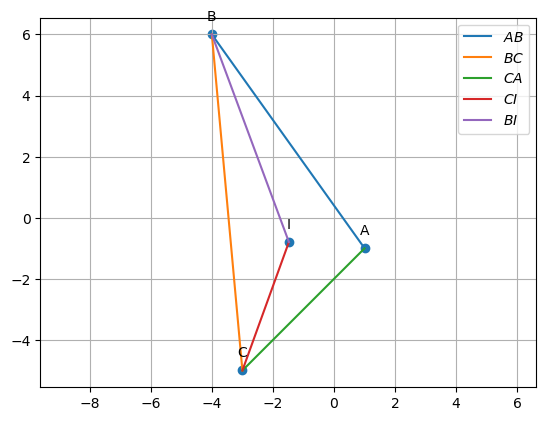
\includegraphics[width=\columnwidth]{./figs/Incentre.png}
\caption{Intersection point $\vec{I}$ of angle bisectors of $\vec{B}$and$\vec{C}$ plotted using python}
\label{fig:i_tri_py}
\end{figure}



	\item Using 
    \eqref{eq:angle2d}
verify that 
		\begin{align}
			\angle BAI = \angle CAI.
		\end{align}
	\item Find the distance from $\vec{I}$ to $BC$.  
	\item Repeat the above exercise for the sides $AB$ and $AC$.
	\item This distance is known as the {\em inradius} $r$.
	\item Draw a circle with center $\vec{I}$ and radius $r$.  $\vec{I}$ is known as the {\em incentre}.
	\item The equation of the {\em incircle} is given by 
		\begin{align}
			\norm{\vec{x}-\vec{I}}^2 = r^2
		\end{align}
		Find the parameteric equation of $BC$ and use it to verify that $BC$ intersects the incircle at exactly one point $\vec{D}_3$.  $BC$ is defined to be a {\em tangent} to the incircle.  $\vec{D}_3$ is defined to be {\em point of contact}.
	\\
		\iffalse
\documentclass[journal,12pt,twocolumn]{IEEEtran}
\usepackage{cite}
\usepackage{amsmath,amssymb,amsfonts,amsthm}
\usepackage{algorithmic}
\usepackage{graphicx}
\usepackage{textcomp}
\usepackage{xcolor}
\usepackage{txfonts}
\usepackage{listings}
\usepackage{enumitem}
\usepackage{mathtools}
\usepackage{gensymb}
\usepackage[breaklinks=true]{hyperref}
\usepackage{tkz-euclide} % loads  TikZ and tkz-base
\usepackage{listings}
\usepackage{float}


\begin{document}
\providecommand{\pr}[1]{\ensuremath{\Pr\left(#1\right)}}
\providecommand{\prt}[2]{\ensuremath{p_{#1}^{\left(#2\right)} }}        % own macro for this question
\providecommand{\qfunc}[1]{\ensuremath{Q\left(#1\right)}}
\providecommand{\sbrak}[1]{\ensuremath{{}\left[#1\right]}}
\providecommand{\lsbrak}[1]{\ensuremath{{}\left[#1\right.}}
\providecommand{\rsbrak}[1]{\ensuremath{{}\left.#1\right]}}
\providecommand{\brak}[1]{\ensuremath{\left(#1\right)}}
\providecommand{\lbrak}[1]{\ensuremath{\left(#1\right.}}
\providecommand{\rbrak}[1]{\ensuremath{\left.#1\right)}}
\providecommand{\cbrak}[1]{\ensuremath{\left\{#1\right\}}}
\providecommand{\lcbrak}[1]{\ensuremath{\left\{#1\right.}}
\providecommand{\rcbrak}[1]{\ensuremath{\left.#1\right\}}}
\newcommand{\sgn}{\mathop{\mathrm{sgn}}}
\providecommand{\abs}[1]{\left\vert#1\right\vert}
\providecommand{\res}[1]{\Res\displaylimits_{#1}} 
\providecommand{\norm}[1]{\left\lVert#1\right\rVert}
%\providecommand{\norm}[1]{\lVert#1\rVert}
\providecommand{\mtx}[1]{\mathbf{#1}}
\providecommand{\mean}[1]{E\left[ #1 \right]}
\providecommand{\cond}[2]{#1\middle|#2}
\providecommand{\fourier}{\overset{\mathcal{F}}{ \rightleftharpoons}}
\newenvironment{amatrix}[1]{%
  \left(\begin{array}{@{}*{#1}{c}|c@{}}
}{%
  \end{array}\right)
}
%\providecommand{\hilbert}{\overset{\mathcal{H}}{ \rightleftharpoons}}
%\providecommand{\system}{\overset{\mathcal{H}}{ \longleftrightarrow}}
	%\newcommand{\solution}[2]{\textbf{Solution:}{#1}}
\newcommand{\solution}{\noindent \textbf{Solution: }}
\newcommand{\cosec}{\,\text{cosec}\,}
\providecommand{\dec}[2]{\ensuremath{\overset{#1}{\underset{#2}{\gtrless}}}}
\newcommand{\myvec}[1]{\ensuremath{\begin{pmatrix}#1\end{pmatrix}}}
\newcommand{\mydet}[1]{\ensuremath{\begin{vmatrix}#1\end{vmatrix}}}
\newcommand{\myaugvec}[2]{\ensuremath{\begin{amatrix}{#1}#2\end{amatrix}}}
\providecommand{\rank}{\text{rank}}
\providecommand{\pr}[1]{\ensuremath{\Pr\left(#1\right)}}
\providecommand{\qfunc}[1]{\ensuremath{Q\left(#1\right)}}
	\newcommand*{\permcomb}[4][0mu]{{{}^{#3}\mkern#1#2_{#4}}}
\newcommand*{\perm}[1][-3mu]{\permcomb[#1]{P}}
\newcommand*{\comb}[1][-1mu]{\permcomb[#1]{C}}
\providecommand{\qfunc}[1]{\ensuremath{Q\left(#1\right)}}
\providecommand{\gauss}[2]{\mathcal{N}\ensuremath{\left(#1,#2\right)}}
\providecommand{\diff}[2]{\ensuremath{\frac{d{#1}}{d{#2}}}}
\providecommand{\myceil}[1]{\left \lceil #1 \right \rceil }
\newcommand\figref{Fig.~\ref}
\newcommand\tabref{Table~\ref}
\newcommand{\sinc}{\,\text{sinc}\,}
\newcommand{\rect}{\,\text{rect}\,}
%%
%	%\newcommand{\solution}[2]{\textbf{Solution:}{#1}}
%\newcommand{\solution}{\noindent \textbf{Solution: }}
%\newcommand{\cosec}{\,\text{cosec}\,}
%\numberwithin{equation}{section}
%\numberwithin{equation}{subsection}
%\numberwithin{problem}{section}
%\numberwithin{definition}{section}
%\makeatletter
%\@addtoreset{figure}{problem}
%\makeatother

%\let\StandardTheFigure\thefigure
\let\vec\mathbf

\bibliographystyle{IEEEtran}


\vspace{3cm}


\title{
Probability Assignment 1	}
}
\author{EE22BTECH11052 - SUJAL GUPTA
	
}	
%\title{
%	\logo{Matrix Analysis through Octave}{\begin{center}\includegraphics[scale=.24]{tlc}\end{center}}{}{HAMDSP}
%}


% paper title
% can use linebreaks \\ within to get better formatting as desired
%\title{Matrix Analysis through Octave}
%
%
% author names and IEEE memberships
% note positions of commas and nonbreaking spaces ( ~ ) LaTeX will not break
% a structure at a ~ so this keeps an author's name from being broken across
% two lines.
% use \thanks{} to gain access to the first footnote area
% a separate \thanks must be used for each paragraph as LaTeX2e's \thanks
% was not built to handle multiple paragraphs
%

%\author{<-this % stops a space
%\thanks{}}
%}
% note the % following the last \IEEEmembership and also \thanks - 
% these prevent an unwanted space from occurring between the last author name
% and the end of the author line. i.e., if you had this:
% 
% \author{....lastname \thanks{...} \thanks{...} }
%                     ^------------^------------^----Do not want these spaces!
%
% a space would be appended to the last name and could cause every name on that
% line to be shifted left slightly. This is one of those "LaTeX things". For
% instance, "\textbf{A} \textbf{B}" will typeset as "A B" not "AB". To get
% "AB" then you have to do: "\textbf{A}\textbf{B}"
% \thanks is no different in this regard, so shield the last } of each \thanks
% that ends a line with a % and do not let a space in before the next \thanks.
% Spaces after \IEEEmembership other than the last one are OK (and needed) as
% you are supposed to have spaces between the names. For what it is worth,
% this is a minor point as most people would not even notice if the said evil
% space somehow managed to creep in.



% The paper headers
%\markboth{Journal of \LaTeX\ Class Files,~Vol.~6, No.~1, January~2007}%
%{Shell \MakeLowercase{\textit{et al.}}: Bare Demo of IEEEtran.cls for Journals}
% The only time the second header will appear is for the odd numbered pages
% after the title page when using the twoside option.
% 
% *** Note that you probably will NOT want to include the author's ***
% *** name in the headers of peer review papers.                   ***
% You can use \ifCLASSOPTIONpeerreview for conditional compilation here if
% you desire.




% If you want to put a publisher's ID mark on the page you can do it like
% this:
%\IEEEpubid{0000--0000/00\$00.00~\copyright~2007 IEEE}
% Remember, if you use this you must call \IEEEpubidadjcol in the second
% column for its text to clear the IEEEpubid mark.



% make the title area
\maketitle

\newpage

%\tableofcontents

\bigskip

\renewcommand{\thefigure}{\theenumi}
\renewcommand{\thetable}{\theenumi}
%\renewcommand{\theequation}{\theenumi}

%\begin{abstract}
%%\boldmath
%In this letter, an algorithm for evaluating the exact analytical bit error rate  (BER)  for the piecewise linear (PL) combiner for  multiple relays is presented. Previous results were available only for upto three relays. The algorithm is unique in the sense that  the actual mathematical expressions, that are prohibitively large, need not be explicitly obtained. The diversity gain due to multiple relays is shown through plots of the analytical BER, well supported by simulations. 
%
%\end{abstract}
% IEEEtran.cls defaults to using nonbold math in the Abstract.
% This preserves the distinction between vectors and scalars. However,
% if the journal you are submitting to favors bold math in the abstract,
% then you can use LaTeX's standard command \boldmath at the very start
% of the abstract to achieve this. Many IEEE journals frown on math
% in the abstract anyway.

% Note that keywords are not normally used for peerreview papers.
%\begin{IEEEkeywords}
%Cooperative diversity, decode and forward, piecewise linear
%\end{IEEEkeywords}



% For peer review papers, you can put extra information on the cover
% page as needed:
% \ifCLASSOPTIONpeerreview
% \begin{center} \bfseries EDICS Category: 3-BBND \end{center}
% \fi
%
% For peerreview papers, this IEEEtran command inserts a page break and
% creates the second title. It will be ignored for other modes.
%\IEEEpeerreviewmaketitle

%\begin{abstract}
%his manual includes \LaTeX figures.
%book provides an introduction to optimization  based on the NCERT textbooks from Class 6-12.  Links to sample Python codes are available in the text.  
%\end{abstract}
%Download 
%\begin{lstlisting}
%svn co https://github.com/gadepall/school/trunk/training
%\end{lstlisting}

%\renewcommand{\theequation}{\theenumi}
%\subsection{Problem}

%\section{Chemistry}
%\begin{enumerate}[label=\arabic*.,ref=\thesection.\theenumi]
%\numberwithin{equation}{enumi}
Given in the question:
% \begin{description}
  % \item 
  \begin{align}
    \vec{A} &= \myvec{1\\-1}  ,\\
  % \item 
    \vec{B} &= \myvec{-4\\6} ,\\
  % \item 
    \vec{C} &= \myvec{-3\\-5}
    \end{align}
% \end{description}

The equation of the incircle is given by
\begin{align}
\norm{\vec{x}-\vec{I}}^2 = r^2
\end{align}
Find the parameteric equation of $BC$ and use it to verify that $BC$
intersects the incircle at exactly one point $\vec{D_{3}}$ . $BC$ is defined to be a
tangent to the incircle. $\vec{D_{3}}$ is defined to be point of contact.
\fi
\solution
Let us define 
\begin{align}
\vec{m} = \vec{C}-\vec{B} 
\end{align}
and $\vec{I}$ is the incentre of the $\triangle ABC$

\begin{align}
\vec{I} &= \frac{1}{\sqrt{74}+\sqrt{32}+\sqrt{122}}\myvec{{\sqrt{122}-4\sqrt{32}-3\sqrt{74}}\\{-\sqrt{122}+6\sqrt{32}-5\sqrt{74}}}\\
&=\myvec{-1.47756217 \\-0.79495069}
\end{align}
The general position vector on the line $BC$ (in parametric form)  and the equation of incircle are:
\begin{align}
\vec{x} &= \vec{B} + k{\vec{m}}\label{eq:8}\\
\norm{\ \vec{x} - \vec{I}\ }^2 &= r^2 \label{eq:9}
\end{align}
Substituting the value of $ \vec{x} $ from \eqref{eq:8} in \eqref{eq:9}
\begin{align}
  \norm{ \vec{B} + k{\vec{m}}- \vec{I} }^2 &= r^2 \\
  \sbrak{\vec{B} + k{\vec{m}}- \vec{I}}^{\top} \sbrak{\vec{B} + k{\vec{m}}- \vec{I}} &= r^2 
\end{align}
On simplifying the above equation:
\begin{multline}
k^2\norm{\vec{m}}^2 +2k{\vec{m}^{\top}}\brak{{\vec{B}-\vec{I}}}+\norm{\vec{I}}^2 +\norm{\vec{B}}^2\\-2\brak{\vec{B}^{\top}\vec{I}} - r^2=0
\end{multline}
The above is a quadratic equation in $k$.
The Discriminant of the quadratic equation is:
\begin{multline}
D = {\cbrak{2\sbrak{\vec{m}^{\top}\brak{\vec{B}-\vec{I}}}}}^2-4(\ \norm{\vec{m}}^2)(\ \norm{\vec{I}}^2 +\norm{\vec{B}}^2\\-2\brak{\vec{B}^{\top}\vec{I}} - r^2)\\
= {\sbrak{2\myvec{1&-11}\myvec{-4+1.47756217\\6+0.79495069}}}^2 \\-4[122][2.8151+52-2(1.140544)\\-3.59820]\\
=4\sbrak{{\brak{-2.522-74.744}}^2-5970.173}\\
=4[5970.173121-5970.173121]\\
=0
\end{multline}
%\end{multline}
%\begin{multline}
%\begin{align}

We substituted the values of $\vec{B},\vec{I},\vec{m}$
On solving this Discriminant turns out to be zero.
Hence, the quadratic equation has only one solution.
To find the unique solution of the equation (i.e. the unique value of $k$), Set discriminant value to 0.
And the solution is \begin{align}k=\frac{-2\vec{m}^{\top}\brak{\vec{B}-\vec{I}}}{2{\ \norm{\vec{m}}^2}}\end{align}

On substituting the values, the value of $k$ is 
\begin{align}
k&=-\myvec{1&-11}\myvec{-4-\frac{\sqrt{122}-4\sqrt{32}-3\sqrt{74}}{\sqrt{74}+\sqrt{32}+\sqrt{122}}\\6-\frac{-\sqrt{122}+6\sqrt{32}-5\sqrt{74}}{\sqrt{74}+\sqrt{32}+\sqrt{122}}}\\
&=\myvec{1&-11}\myvec{\frac{5\sqrt{122}+\sqrt{74}}{\sqrt{74}+\sqrt{32}+\sqrt{122}}\\\frac{-7\sqrt{122}-11\sqrt{74}}{\sqrt{74}+\sqrt{32}+\sqrt{122}}}\\
&=\frac{122\sqrt{74}+82\sqrt{122}}{122(\sqrt{74}+\sqrt{122}+\sqrt{32})}\\
&=0.6333352080102638
\end{align}

So on substituting this value in \eqref{eq:8}, we get the point $\vec{D_{3}}$ 
\begin{align}
\vec{D_{3}} &=\myvec{-4\\6} + \frac{122\sqrt{74}+82\sqrt{122}}{122\brak{\sqrt{74}+\sqrt{122}+\sqrt{32}}}\myvec{1\\-11}\\
&=\myvec{-4+\frac{122\sqrt{74}+82\sqrt{122}}{122\brak{\sqrt{74}+\sqrt{122}+\sqrt{32}}}\\6-11\frac{122\sqrt{74}+82\sqrt{122}}{122\brak{\sqrt{74}+\sqrt{122}+\sqrt{32}}}}\\
&=\myvec{{\frac{-366\sqrt{74}-406\sqrt{122}-488\sqrt{32}}{122\brak{\sqrt{74}+\sqrt{32}+\sqrt{122}}}}\\{\frac{-610\sqrt{74}+732\sqrt{32}-170\sqrt{122}}{122\brak{\sqrt{74}+\sqrt{32}+\sqrt{122}}}}}\\
&=\myvec{-3.36666479\\-0.96668729}
\end{align}

\begin{figure}[H]
\centering
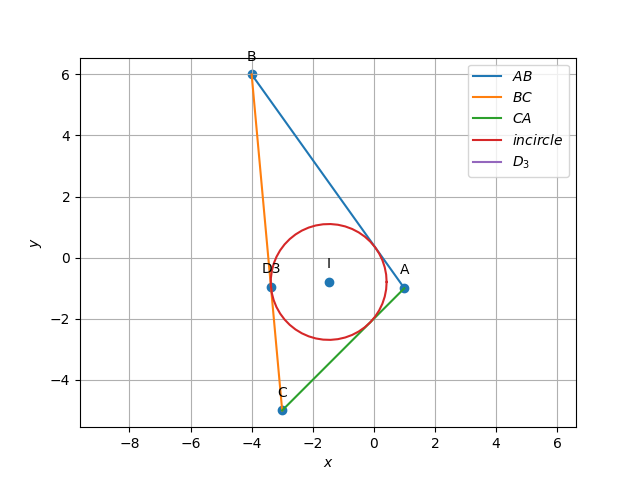
\includegraphics[width=\columnwidth]{solutions/1/5/8/figs/incircle.png}
\caption{Incircle generated using python}
\label{fig:Incircle_py}
\end{figure}

  \item Find the other points of contact $\vec{E}_3$ and $\vec{F}_3$.
	\item Verify that 
		\begin{align}
			AE_3 = AF_3=m, BD_3 = BF_3=n, CD_3 = CE_3=p.
		\end{align}
	\item Obtain $m,n,p$ in terms of $a,b,c$, the sides of the triangle using a matrix equation.  Obtain the numerical values.
 \\
 		
\let\negmedspace\undefined
\let\negthickspace\undefined
\documentclass[journal,12pt,twocolumn]{IEEEtran}
\usepackage{cite}
\usepackage{amsmath,amssymb,amsfonts,amsthm}
\usepackage{algorithmic}
\usepackage{graphicx}
\usepackage{textcomp}
\usepackage{xcolor}
\usepackage{txfonts}
\usepackage{listings}
\usepackage{enumitem}
\usepackage{mathtools}
\usepackage{gensymb}
\usepackage[breaklinks=true]{hyperref}
\usepackage{tkz-euclide} % loads  TikZ and tkz-base
\usepackage{listings}
\usepackage{gvv}
%
%\usepackage{setspace}
%\usepackage{gensymb}
%\doublespacing
%\singlespacing

%\usepackage{graphicx}
%\usepackage{amssymb}
%\usepackage{relsize}
%\usepackage[cmex10]{amsmath}
%\usepackage{amsthm}
%\interdisplaylinepenalty=2500
%\savesymbol{iint}
%\usepackage{txfonts}
%\restoresymbol{TXF}{iint}
%\usepackage{wasysym}
%\usepackage{amsthm}
%\usepackage{iithtlc}
%\usepackage{mathrsfs}
%\usepackage{txfonts}
%\usepackage{stfloats}
%\usepackage{bm}
%\usepackage{cite}
%\usepackage{cases}
%\usepackage{subfig}
%\usepackage{xtab}
%\usepackage{longtable}
%\usepackage{multirow}
%\usepackage{algorithm}
%\usepackage{algpseudocode}
%\usepackage{enumitem}
%\usepackage{mathtools}
%\usepackage{tikz}
%\usepackage{circuitikz}
%\usepackage{verbatim}
%\usepackage{tfrupee}
%\usepackage{stmaryrd}
%\usetkzobj{all}
%    \usepackage{color}                                            %%
%    \usepackage{array}                                            %%
%    \usepackage{longtable}                                        %%
%    \usepackage{calc}                                             %%
%    \usepackage{multirow}                                         %%
%    \usepackage{hhline}                                           %%
%    \usepackage{ifthen}                                           %%
  %optionally (for landscape tables embedded in another document): %%
%    \usepackage{lscape}     
%\usepackage{multicol}
%\usepackage{chngcntr}
%\usepackage{enumerate}

%\usepackage{wasysym}
%\documentclass[conference]{IEEEtran}
%\IEEEoverridecommandlockouts
% The preceding line is only needed to identify funding in the first footnote. If that is unneeded, please comment it out.

\newtheorem{theorem}{Theorem}[section]
\newtheorem{problem}{Problem}
\newtheorem{proposition}{Proposition}[section]
\newtheorem{lemma}{Lemma}[section]
\newtheorem{corollary}[theorem]{Corollary}
\newtheorem{example}{Example}[section]
\newtheorem{definition}[problem]{Definition}
%\newtheorem{thm}{Theorem}[section] 
%\newtheorem{defn}[thm]{Definition}
%\newtheorem{algorithm}{Algorithm}[section]
%\newtheorem{cor}{Corollary}
\newcommand{\BEQA}{\begin{eqnarray}}
\newcommand{\EEQA}{\end{eqnarray}}
\newcommand{\define}{\stackrel{\triangle}{=}}
\theoremstyle{remark}
\newtheorem{rem}{Remark}

%\bibliographystyle{ieeetr}
\begin{document}
%

\bibliographystyle{IEEEtran}


\vspace{3cm}

\title{
    Solution to problem number 1.5.11
}
\author{ Yash Patil - EE22BTECH11058}
%\title{
%	\logo{Matrix Analysis through Octave}{\begin{center}\includegraphics[scale=.24]{tlc}\end{center}}{}{HAMDSP}
%}


% paper title
% can use linebreaks \\ within to get better formatting as desired
%\title{Matrix Analysis through Octave}
%
%
% author names and IEEE memberships
% note positions of commas and nonbreaking spaces ( ~ ) LaTeX will not break
% a structure at a ~ so this keeps an author's name from being broken across
% two lines.
% use \thanks{} to gain access to the first footnote area
% a separate \thanks must be used for each paragraph as LaTeX2e's \thanks
% was not built to handle multiple paragraphs
%

%\author{<-this % stops a space
%\thanks{}}
%}
% note the % following the last \IEEEmembership and also \thanks - 
% these prevent an unwanted space from occurring between the last author name
% and the end of the author line. i.e., if you had this:
% 
% \author{....lastname \thanks{...} \thanks{...} }
%                     ^------------^------------^----Do not want these spaces!
%
% a space would be appended to the last name and could cause every name on that
% line to be shifted left slightly. This is one of those "LaTeX things". For
% instance, "\textbf{A} \textbf{B}" will typeset as "A B" not "AB". To get
% "AB" then you have to do: "\textbf{A}\textbf{B}"
% \thanks is no different in this regard, so shield the last } of each \thanks
% that ends a line with a % and do not let a space in before the next \thanks.
% Spaces after \IEEEmembership other than the last one are OK (and needed) as
% you are supposed to have spaces between the names. For what it is worth,
% this is a minor point as most people would not even notice if the said evil
% space somehow managed to creep in.



% The paper headers
%\markboth{Journal of \LaTeX\ Class Files,~Vol.~6, No.~1, January~2007}%
%{Shell \MakeLowercase{\textit{et al.}}: Bare Demo of IEEEtran.cls for Journals}
% The only time the second header will appear is for the odd numbered pages
% after the title page when using the twoside option.
% 
% *** Note that you probably will NOT want to include the author's ***
% *** name in the headers of peer review papers.                   ***
% You can use \ifCLASSOPTIONpeerreview for conditional compilation here if
% you desire.




% If you want to put a publisher's ID mark on the page you can do it like
% this:
%\IEEEpubid{0000--0000/00\$00.00~\copyright~2007 IEEE}
% Remember, if you use this you must call \IEEEpubidadjcol in the second
% column for its text to clear the IEEEpubid mark.



% make the title area
\maketitle

\newpage

%\tableofcontents

\bigskip

\renewcommand{\thefigure}{\theenumi}
\renewcommand{\thetable}{\theenumi}
%\renewcommand{\theequation}{\theenumi}

%\begin{abstract}
%%\boldmath
%In this letter, an algorithm for evaluating the exact analytical bit error rate  (BER)  for the piecewise linear (PL) combiner for  multiple relays is presented. Previous results were available only for upto three relays. The algorithm is unique in the sense that  the actual mathematical expressions, that are prohibitively large, need not be explicitly obtained. The diversity gain due to multiple relays is shown through plots of the analytical BER, well supported by simulations. 
%
%\end{abstract}
% IEEEtran.cls defaults to using nonbold math in the Abstract.
% This preserves the distinction between vectors and scalars. However,
% if the journal you are submitting to favors bold math in the abstract,
% then you can use LaTeX's standard command \boldmath at the very start
% of the abstract to achieve this. Many IEEE journals frown on math
% in the abstract anyway.

% Note that keywords are not normally used for peerreview papers.
%\begin{IEEEkeywords}
%Cooperative diversity, decode and forward, piecewise linear
%\end{IEEEkeywords}



% For peer review papers, you can put extra information on the cover
% page as needed:
% \ifCLASSOPTIONpeerreview
% \begin{center} \bfseries EDICS Category: 3-BBND \end{center}
% \fi
%
% For peerreview papers, this IEEEtran command inserts a page break and
% creates the second title. It will be ignored for other modes.
%\IEEEpeerreviewmaketitle
\textbf{Question:}
Obtain p, q, r in terms of a, b, c, the sides of the triangle using a matrix
equation. Obtain the numerical values.\\
\indent\textbf{Solution:}
Given in the question:
\begin{align}
    \vec{A} &= \myvec{ 1 \\ -1 }\\
    \vec{B} &= \myvec{ -4 \\ 6 }\\
    \vec{C} &= \myvec{ -3 \\ -5 } 
\end{align}
Now, the side lengths a, b and c can be calculated as:
\begin{align}
    a &= \sqrt{(\vec{C}-\vec{B})^{\top}(\vec{C}-\vec{B})}\\
    &= \sqrt{\myvec{1&-11} \myvec{1\\-11}}\\
    &= \sqrt{1+121}\\
    &=\sqrt{122}    \\
    b &= \sqrt{(\vec{A}-\vec{C})^{\top}(\vec{A}-\vec{C})}\\
    &= \sqrt{\myvec{4&4} \myvec{4\\4}}\\
    &= \sqrt{16+16}\\
    &=\sqrt{32}     \\
    c &= \sqrt{(\vec{B}-\vec{A})^{\top}(\vec{B}-\vec{A})}\\
    &= \sqrt{\myvec{-5&7} \myvec{-5\\7}}\\
    &= \sqrt{25+49}\\
    &=\sqrt{74}
\end{align}
AB being a straight line with $F_3$ a point on it, it can be said that
\begin{align}
    AB &= AF_3 + BF_3\\
    BC &= BD_3 + CD_3\\
    CA &= AE_3 + BE_3\\
% 
    \therefore 
    c &= m+n,\\
    a &= n+p, \\
    b &= m+p 
\end{align}
these 3 equations can be written as:
\begin{align}
    \myvec{1&1&0\\0&1&1\\1&0&1\\}\myvec{m\\n\\p} &= \myvec{1&0&0\\0&1&0\\0&0&1}\myvec{c\\a\\b}\\
    \implies\myvec{1&1&0\\0&1&1\\1&0&1\\}\myvec{m\\n\\p} &= \myvec{c\\a\\b}
\end{align}
solving by row reduction method,
\begin{align}
    \myvec{1&1&0&c\\0&1&1&a\\1&0&1&b}\\
    \xleftrightarrow[]{R_1 \leftarrow R_1+R_3-R_2}&
    \myvec{2&0&0&c+b-a\\0&1&1&a\\1&0&1&b}\\
    \xleftrightarrow[]{R_1 \leftarrow \frac{R_1}{2}}&
    \myvec{1&0&0&\frac{c+b-a}{2}\\0&1&1&a\\1&0&1&b}\\
    \xleftrightarrow[]{R_3 \leftarrow R_3-R_1}&
    \myvec{1&0&0&\frac{c+b-a}{2}\\0&1&1&a\\0&0&1&\frac{a+b-c}{2}}\\
    \xleftrightarrow[]{R_2 \leftarrow R_2-R_3}&
    \myvec{1&0&0&\frac{c+b-a}{2}\\0&1&0&\frac{a+c-b}{2}\\0&0&1&\frac{a+b-c}{2}}
\end{align}
\begin{align}
    \therefore
    m&=\frac{c+b-a}{2}\\ 
    &=\frac{\sqrt{74}+\sqrt{32}-\sqrt{122}}{2}\\
    n&=\frac{a+c-b}{2}\\ 
    &=\frac{\sqrt{74}+\sqrt{122}-\sqrt{32}}{2}\\
    p&=\frac{a+b-c}{2}\\
    &=\frac{\sqrt{122}+\sqrt{32}-\sqrt{74}}{2}
\end{align}

\end{document}

\end{enumerate}
